\documentclass[twoside, a4paper, 10pt]{report}
\usepackage[italian]{babel}
\usepackage[utf8]{inputenc}
\usepackage[margin=1in]{geometry}
\usepackage{graphicx}
\usepackage{fancyhdr}
\usepackage{array}
\usepackage{colortbl}
\usepackage{lastpage}
\usepackage{titlesec}
\usepackage{float}
\usepackage{subcaption}
\usepackage{hyperref}
\usepackage{afterpage}

% Ridefinizione per il titolo dei capitoli
\titleformat{\chapter}[hang]{\LARGE\bfseries}{\thechapter}{1em}{} 
\titlespacing{\chapter}{0pt}{0pt}{1em}

% Definizione della path per le immagini
\graphicspath{{../images/}}

% Set the version of the document
\newcommand{\version}{0.2}
\newcommand{\ProjectTitle}{SatisTrento}
\newcommand{\ProjectTitleShort}{satisTrento}
\newcommand{\FileName}{D2-\ProjectTitleShort-analisiProgettazione}

% Definizione dei dati del documento
\title{Analisi e Progettazione - \ProjectTitle}
\author{Facchini Luca, Prigione Luca, Faa Enrico}
\date{A.A. 2024/2025}

% Definizione metadati PDF
\hypersetup{
    pdftitle={\ProjectTitle},
    pdfauthor={Facchini Luca, Prigione Luca, Faa Enrico},
    pdfsubject={Analisi e Progettazione},
    pdfkeywords={\ProjectTitle, Analisi e Progettazione, Comune di Trento, UniTN}
}

% Rimozione scritta "Capitolo" dai titoli dei capitoli
\renewcommand{\chaptermark}[1]{%
    \markboth{
        \thechapter.\ #1%
    }{}%
}
% Definizione del layout della pagina
\fancypagestyle{stdPage}{
    \setlength{\headheight}{24.0pt} 
    \renewcommand{\footrulewidth}{0.4pt}
    \fancyhead{}
    \fancyfoot{}
    \fancyhead[LE,RO]{\begin{tabular}{l l}
        \textbf{Document:} & Descrizione di progetto \\
        \textbf{Version:} & \version
    \end{tabular}}
    \fancyfoot[LE,RO]{\thepage / \pageref*{LastPage}}
    \fancyhead[LO,RE]{\leftmark}
}
\fancypagestyle{plain}{
    \pagestyle{stdPage}
}
\fancypagestyle{index}{
    \pagestyle{stdPage}
    \fancyfoot[LE,RO]{\thepage}
}

\fancypagestyle{emptyPage}{
    \setlength{\headheight}{24.0pt} 
    \renewcommand{\headrulewidth}{0pt}
    \fancyhead{}
    \fancyfoot{}
}

% Definizione della pagina bianca
\newcommand\blankpage{%
    \null
    \thispagestyle{empty}%
    \addtocounter{page}{-1}%
    \newpage}

\begin{document}
    \pagestyle{fancy}
    \pagenumbering{Roman} 
    
    \begin{titlepage}
        \thispagestyle{emptyPage}
        
\includegraphics[width=0.33\textwidth]{logoUni.png}
        \vspace{1cm}\newline
        \textbf{Progetto:}
        \vspace{0.5cm}
        \begin{center}
            \textbf{\Huge{\ProjectTitle}}
        \end{center}
        \vspace{1cm}
        \textbf{Titolo del documento:}
        \vspace{0.5cm}
        \begin{center}
            \textbf{\huge{Analisi e Progettazione}}
        \end{center}
        \vspace{1cm}
        \textbf{Document Info}
        \vspace{0.5cm}
        % Table with document info
        \begin{center}
            \begin{tabular}{|l|l|l|c|}  
                \hline
                {\cellcolor[rgb]{0,0.502,1}}\textcolor{white}{\textbf{Doc. Name}}   & \FileName & {\cellcolor[rgb]{0,0.502,1}}\begin{tabular}[c]{@{}>{\cellcolor[rgb]{0,0.502,1}}l@{}}\textcolor{white}{\textbf{Doc.}}\\\textcolor{white}{\textbf{Number}}\end{tabular} & D2 V\version  \\ 
                \hline
                {\cellcolor[rgb]{0,0.502,1}}\textcolor{white}{\textbf{Description}} & \multicolumn{3}{l|}{Documento di analisi dei requisiti funzionali, non funzionali e front-end}                                                                                                                               \\
                \hline
            \end{tabular}
        \end{center}
        % Document authors (1 per line) with name and ID aligned to the right but with some space from the right border 
        \vspace{1.5in}
        \vfill
        \begin{flushright}
            \rightskip=2cm
            \begin{tabular}{r l}
                \multicolumn{2}{c}{\textbf{Authors}} \\
                Facchini Luca & 245965 \\
                Prigione Luca & 242880 \\
                Faa Enrico & 243889
            \end{tabular}
        \end{flushright}
        \vfill
    \end{titlepage}
    % \afterpage{\blankpage} % Uncomment this line if to print as a booklet
    \begingroup
        \setcounter{tocdepth}{0}
        \tableofcontents
        \thispagestyle{index}
    \endgroup
    \pagestyle{stdPage}
    % \afterpage{\blankpage} % Uncomment this line if to print as a booklet
    \newpage
    \pagenumbering{arabic} 
    
    \chapter{Requisiti Funzionali}
\label{ch:requisitiFunzionali}

Di seguito vengono riportati i requisiti funzionali (\texttt{RF}) del programma "SatisTrento" tramite \textit{Use Case Diagram} (\texttt{UCD}) progettati usando il linguaggio \texttt{UML}.

% Esempio di markup
\section{\underline{Utente non loggato}}
    Di seguito i requisiti associati all'Utente non loggato:
    \begin{itemize}
        \item \textbf{RF1}: Visualizzazione città
        \item \textbf{RF2}: Interazione con la mappa
        \item \textbf{RF3}: Visualizzazione zona
        \item \textbf{RF4}: Elenco strutture
        \item \textbf{RF5}: Multi lingua
        \item \textbf{RF6}: Login
    \end{itemize}
    \begin{figure}[H]
        \centering
        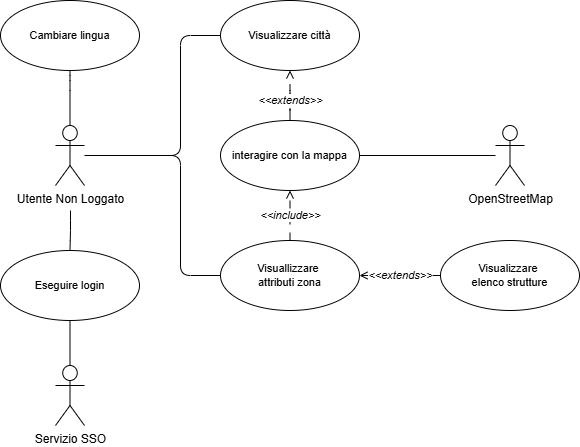
\includegraphics[width=0.8\textwidth]{UseCase_diagrams/NonLoggato.drawio.png}
        \caption{Use Case Diagram dell'Utente non loggato}
    \end{figure}

    \subsection{Visualizzare città}
        \subsubsection{Riassunto}
            Questo Use Case descrive come l'utente può visualizzare gli attributi e la mappa della città
        \subsubsection{Descrizione}
            \begin{itemize}
                \item Il sistema mostra nella parte sinistra dello schermo gli attributi demografici e riguardanti la soddisfazione della città
                \item Il sistema mostra nella parte destra dello schermo la mappa della città suddivisa nella zona selezionata (Estensione 1)
            \end{itemize}
        \subsubsection{Estensioni}
            \begin{itemize}
                \item La tipologia di zona selezionata di default è quella dei quartieri
            \end{itemize}
    
    \subsection{Interagire con la mappa}
        \subsubsection{Riassunto}
            Questo Use Case descrive come l'utente può interagire con la mappa
        \subsubsection{Descrizione}
            \begin{itemize}
                \item L'utente non loggato posiziona il cursone all'interno dello spazio dedicato alla mappa
                \item Se l'utente utilizza la rotella del mouse oppure uno dei pulsanti presenti in uno degli angoli della mappa
                \item Attraverso le funzionalità fornite da OpenStreetMap la mappa ingrandisce o diminuisce la dimensione dello zoom (Eccezione 1)
                \item Se l'utente preme e trascina il cursore
                \item Attraverso le funzionalità fornite da OpenStreetMap la mappa sposta il focus centrale in funzione del cursore (Eccezione 2)
                \item Se l'utente non loggato seleziona una delle zone all'interno della visuale della mappa (Estensione 1)
                \item Il sistema posiziona il focus centrale della mappa al centro della zona selezionata e ne modifica successivamente lo zoom, il colore e lo spessore dei bordi
                \item Il sistema passa successivamente allo UseCase "Visualizzare zona" della sezione scelta
            \end{itemize}
        \subsubsection{Eccezioni}
            \begin{enumerate}
                \item Nel caso in cui l'utente non loggato cercasse di aumentare o diminuire lo zoom oltre ai limiti imposti, il sistema deve bloccare la nuova modifica allo zoom
                \item Nel caso in cui l'utente non loggato cercasse di spostare il focus centrale oltre ai limiti della città, il sistema deve bloccare la nuova modifica allo spostamento del focus centrale
            \end{enumerate}
        \subsubsection{Estensioni}
            \begin{enumerate}
                \item Nel caso in cui l'utente cliccasse su di una zona già selezionata questa riporterebbe allo UseCase "Visualizzare città"
                \item L'utente, selezionando il pulsante presente nell'angolo della mappa, potrà visualizzare un menù a pop-up e successivamente modificare la tipologia di divisione presente all'interno della mappa
            \end{enumerate}
    
    \subsection{Visualizzare zona}
        \subsubsection{Riassunto}
            Questo Use Case descrive come l'utente può visualizzare la zona selezionata della città
        \subsubsection{Descrizione}
            \begin{enumerate}
                \item Dopo aver interagito con la mappa ed aver selezionato una zona
                \item Il sistema mostra nella parte sinistra dello schermo la mappa centrata sul centro della zona selezionata
                \item Il sistema mostra nella parte destra dello schermo gli attributi demografici e riguardanti la soddisfazione della zona della città selezionata
            \end{enumerate}

    \subsection{Visualizzare elenco strutture}
        \subsubsection{Riassunto}
            Questo Use Case descrive come l'utente può accedere e visualizzare l'elenco delle strutture che forniscono un servizio al cittadino
        \subsubsection{Descrizione}
            \begin{enumerate}
                \item L'utente non loggato preme uno degli attributi presenti a schermo (Eccezione 1)
                \item Il sistema presenta a schermo, ove prima erano presenti gli attributi riguardanti la zona selezionata, una tabella contenente una lista numerata di strutture che offrono il servizio selezionato in precedenza
                \item Il sistema deve successivamente segnalare sulla mappa la posizione delle varie strutture, attraverso un segnalino contenente il numero identificativo presente in tabella della struttura
            \end{enumerate}
        \subsubsection{Eccezioni}
            \begin{enumerate}
                \item Nel caso in cui per una tipologia di dato non fossero presenti strutture il sistema non deve fare nulla
            \end{enumerate}
        \subsubsection{Estensioni}
            \begin{enumerate}
                \item Nel caso in cui l'utente cliccasse il pulante per chiudere la tabella il sistema tornerà alla visualizzazione della zona selezionata in precedenza
            \end{enumerate}

    \subsection{Cambiare lingua}
        \subsubsection{Riassunto}
            Questo Use Case descrive come l'utente può cambiare la lingua dei vari testi presenti nel programma
        \subsubsection{Descrizione}
            \begin{enumerate}
                \item L'utente preme sul menù a tendina presente nella header e seleziona la sezione riguardante la modifica della lingua
                \item Il sistema presenterà a schermo un menù pop-up contenente la lista di lingue per le quali è disponibile la traduzione
                \item Se l'utente seleziona la lingua e clicca il pulsante di conferma (Eccezione 1 e 2)
                \item Il sistema ricarica la pagina selezionata con i testi nella lingua selezionata
            \end{enumerate}
        \subsubsection{Eccezioni}
            \begin{enumerate}
                \item Nel caso in cui l'utente non loggato selezionasse e confermasse la lingua già selezionata, il sistema deve chiudere il pop-up senza apportare alcuna modifica
            \end{enumerate}

    \subsection{Eseguire login}
        \subsubsection{Riassunto}
            Questo Use Case descrive come l'utente non loggato può eseguire il login
        \subsubsection{Descrizione}
            \begin{enumerate}
                \item L'utente preme sul menù a tendina presente all'interno della header e seleziona la sezione riguardante il login
                \item Il sistema reindirizza l'utente alla pagina del service provider della provincia di Trento dal quale potrà accedere al login tramite sistema SSO
                \item Il sistema SSO verifica l'identità dell'utente in questione e la ritorna al sistema (Eccezione 1)
                \item Il sistema controlla che per l'identità certificata dal sistema SSO esista un'account collegato (Eccezione 1)
                \item Il sistema assegna dunque un'identità all'utente assegnandogli il ruolo di proprietà
                \item Il sistema successivamente al login sostituisce l'icona del login con l'immagine profilo dell'account al quale si ha fatto l'accesso e reindirizza l'utente allo UseCase "visualizzare città"
            \end{enumerate}
        \subsubsection{Eccezioni}
            \begin{enumerate}
                \item Nel caso in cui l'autenticazione fallisse o non vi fossero account collegati il sistema ritorna alla pagina dalla quale si ha provato a fare il login
            \end{enumerate}


\section{\underline{Utente Sondaggista}}
    Di seguito i requisiti associati all'Utente Sondaggista:
    \begin{itemize}
        \item \textbf{RF7}: Logout
        \item \textbf{RF8}: Visualizzazione sondaggi
        \item \textbf{RF9}: Gestione sondaggi
        \item \textbf{RF10}: Visualizzazione voti
        \item \textbf{RF11}: Gestione voti
    \end{itemize}
    \begin{figure}[H]
        \centering
        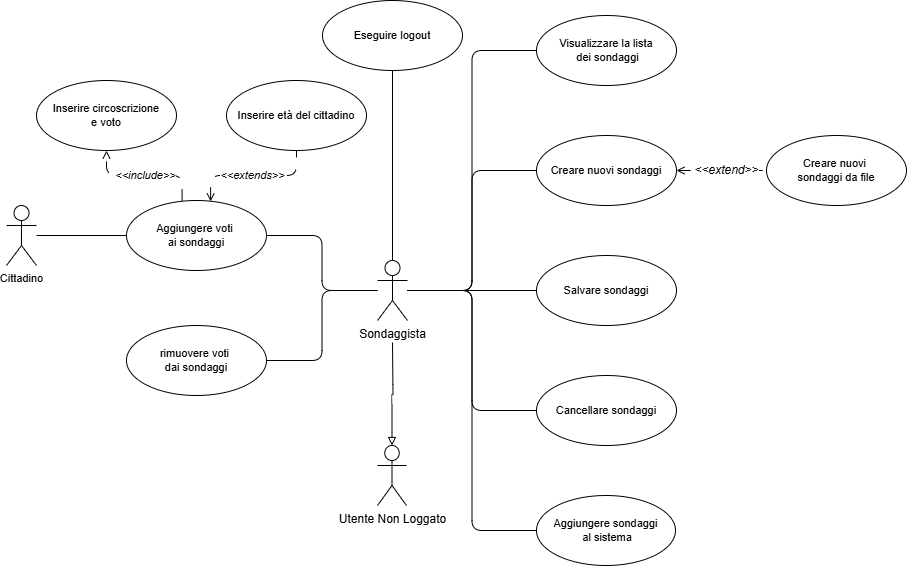
\includegraphics[width=0.8\textwidth]{UseCase_diagrams/Sondaggista.drawio.png}
        \caption{Use Case Diagram dell'Utente sondaggista}
    \end{figure}

    \subsection{Logout}
        \subsubsection{Riassunto}
            Questo Use Case descrive come l'utente può fare logout
        \subsubsection{Descrizione}
            \begin{enumerate}
                \item L'utente sondaggista preme sul menù a tendina presente all'interno della header e seleziona la sezione riguardante il logout
                \item Il sistema scollega lo user dall'account al quale era collegato riportandolo allo stato di utente non loggato, infine 
                ricarica la pagina riportando l'utente alla 'visualizzazione città'
            \end{enumerate}

    \subsection{Visualizzare i sondaggisti}
        \subsubsection{Titolo}
            Questo Use Case descrive come l'utente sondaggista visualizzerà i sondaggi e le interfacce per gestirli
        \subsubsection{Descrizione}
            \begin{enumerate}
                \item Il sistema mostra nel riquadro in alto a sinistra dello schermo l'interfaccia per la creazione di nuovi sondaggi con relative caselle di testo e pulsante per la creazione
                \item Il sistema mostra nel riquadro in basso a sinistra dello schermo l'interfaccia per il caricamento dei sondaggi attraverso pulsante o "drag and drop"
                \item Il sistema mostra nel riquadro in alto a destra dello schermo l'elenco dei sondaggi non ancora caricati, o in fase di caricamento, a sistema con relativo stato della sessione (Eccezione 1)
                \item Il sistema mostra nel riquadro in basso a destra dello schermo l'elenco dei sondaggi già caricati a sistema con relativo stato di caricamento e stato di verifica dei dati inseriti (Eccezione 1)
            \end{enumerate}
        \subsubsection{Eccezioni}
            \begin{enumerate}
                \item Nel caso in cui non fossero presenti sondaggi all'interno di uno degli elenchi il sistema mostrerà a schermo un messaggio per avvisare che tale sezione risulta vuota
            \end{enumerate}

    \subsection{Gestione sonaggi}

    \subsection{Visualizzare i voti}
        \subsubsection{Titolo}
            Questo Use Case descrive come l'utente sondaggista visualizzerà i voti e le interfacce per gestirli
        \subsubsection{Descrizione}
            \begin{enumerate}
                \item Il sistema mostra nella parte sinistra dello schermo un riassunto del numero di voti presenti all'interno del sondaggio e in basso una tabella riassuntiva riguardante il numero di voti ricevuti per quartiere
                \item Il sistema mostra nel riquadro in alto a destra dello schermo l'interfaccia per il caricamento dei voti con le corrispettive caselle di testo
                \item Il sistema mostra nel riquadro in basso a destra dello schermo l'interfaccia per la gestione dei sondaggi
                \item Il sistema mostra nel riquadro in basso al centro dello schermo l'elenco dei voti caricati in precedenza, su ogni voto è inoltre presente l'id, l'ora al quale è stato caricato il voto e infine il pulsante per eliminarlo (Eccezione 1)
            \end{enumerate}
        \subsubsection{Eccezioni}
            \begin{enumerate}
                \item Nel caso in cui non fossero presenti voti all'interno della lista il sistema mostrerà a schermo un messaggio per avvisare che tale sezione risulta vuota
            \end{enumerate}

    \subsection{Gestione voti}
    
    % \afterpage{\blankpage} % Uncomment this line if to print as a booklet
\end{document}